\fenicschapter{UFC: a finite element code generation interface}
              {UFC}
              {Martin Sandve Aln\ae{}s, Anders Logg and Kent-Andre Mardal}
              {alnes-2}

A central component of FEniCS is the UFC interface (Unified
Form-assembly Code). UFC is an interface between problem-specific and
general-purpose components of finite element programs. In particular,
the UFC interface defines the structure and signature of the code that
is generated by the form compilers FFC and SFC for DOLFIN.
The UFC interface applies to a wide range of finite element problems
(including mixed finite elements and discontinuous Galerkin methods)
and may be used with libraries that differ widely in their design. For
this purpose, the interface does not depend on any other FEniCS
components (or other libraries) and consists only of a minimal set of
abstract C++ classes using plain C arrays for data transfer.
This chapter gives a short overview of the UFC interface. For a more
comprehensive discussion, we refer to the UFC
manual~\citep{AlnaesLangtangenEtAl2007} and the
paper~\citet{AlnaesLoggMardalEtAl2009}.

%------------------------------------------------------------------------------
\section{Overview}
\label{sec:alnes-2overview}

A key step in the solution of partial differential equations by the
finite element method is the assembly of linear and nonlinear systems
of equations. The implementation of such solvers is much helped by the
existence of generic software libraries that provide data structures
and algorithms for computational meshes and linear algebra. This
allows the implementation of a generic assembly algorithm that may be
partly reused from one application to another. However, since the
inner loop of the assembly algorithm inherently depends on the partial
differential equation being solved and the finite elements used to
produce the discretization, this inner loop must typically be supplied
by the user. Writing the inner loop is a challenging task that is
prone to errors, and which prohibits rapid prototyping and
experimentation with models and discretization methods.

The FEniCS toolchain of FIAT--UFC--FFC/SFC--UFC--DOLFIN is an attempt
to solve this problem. By generating automatically the inner loop
based on a high-level description of the finite element variational
problem (in the UFL form language), FEniCS is able to provide a
completely generic implementation of the assembly algorithm as part of
DOLFIN. This is illustrated in
Figure~\ref{fig:alnes-2:ufc_flowdiagram}. We note from this figure
that the user input is partitioned into two sets: a first subset
consisting of the finite element variational problem that requires
code generation, and a second subset consisting of the mesh and
coefficient data that is given as input to the assembler.

\begin{figure}
  \ffigbox{\caption{A flow diagram of finite element assembly in FEniCS.}
           \label{fig:alnes-2:ufc_flowdiagram}}
          {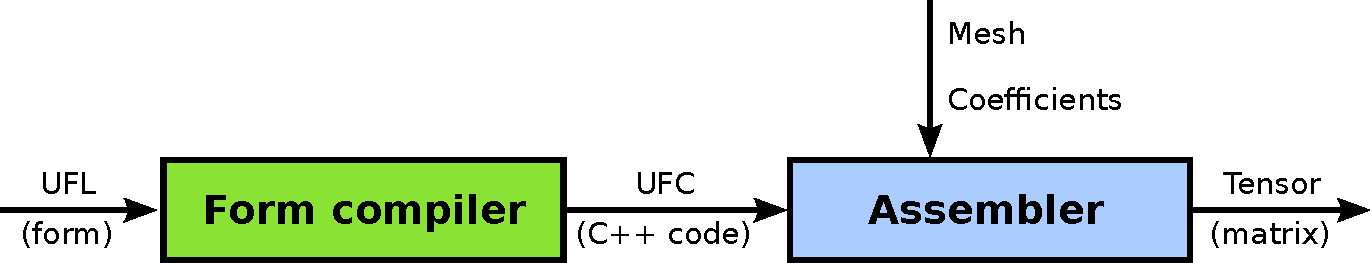
\includegraphics[width=\fullfig]{chapters/alnes-2/pdf/ufc_flowdiagram.pdf}}
\end{figure}

%------------------------------------------------------------------------------
\section{Finite element discretization and assembly}
\label{sec:alnes-2fem}

In Chapter~\ref{chap:logg-3}, we described the assembly algorithm for
computing the global rank~$\rho$ tensor~$A$ corresponding to a
multilinear form~$a$ of arity~$\rho$:
\begin{equation} \label{eq:varform}
  \begin{split}
    a &: W_{1,h} \times W_{2,h} \times \cdots \times W_{n,h} \, \times \,
    V_{\rho,h} \times \cdots \times V_{2,h} \times V_{1,h} \rightarrow \R, \\
    a &\mapsto a(w_1, w_2, \ldots, w_n; v_{\rho}, \ldots, v_2, v_1);
  \end{split}
\end{equation}
Here, $\{V_{j,h}\}_{j=1}^{\rho}$ is a sequence of discrete function
spaces for the \emph{arguments} $\{v_j\}_{j=1}^{\rho}$ of the form and
$\{W_{j,h}^j\}_{j=1}^n$ is a sequence of discrete function spaces for
the \emph{coefficients} $\{w_j\}_{j=1}^n$ of the form. Typically, the
arity is $\rho=1$ for a linear form or $\rho=2$ for a bilinear
form. In the simplest case, all function spaces are equal but there
are many important examples, such as mixed methods, where the
arguments come from different function spaces. The choice of
coefficient function spaces depends on the application; a polynomial
basis simplifies exact integration, while in some cases evaluating
coefficients in quadrature points may be required.

As we saw in Chapter~\ref{chap:logg-3}, the global tensor~$A$ can be
computed by summing contributions from the cells and facets of a
mesh. We refer to these contributions as either \emph{cell tensors} or
\emph{facet tensors}. Although one may formulate a generic assembly
algorithm, the cell and facet tensors must be computed differently
depending on the variational form, and their entries must be inserted
differently into the global tensor depending on the choice of finite
element spaces. This is handled in FEniCS by implementing a generic
assembly algorithm (as part of DOLFIN) that relies on special-purpose
generated code (by FFC or SFC) for computing the cell and facet
tensors, and for computing the local-to-global map for insertion of
the cell and facet tensors into the global matrix.

The UFC interface assumes that the multilinear form~$a$
in~\eqref{eq:varform} can be expressed as a sum of integrals over the
cells~$\mathcal{T}_h$, the exterior facets~$\partial_h$, and the
interior facets~$\partial_h^0$ of the mesh. The integrals may then be
expressed on disjoint subsets $\mathcal{T}_h = \cup_{k=1}^{n_c}
\mathcal{T}_{h,k}$, $\partial_h = \cup_{k=1}^{n_f} \partial_{h,k}$,
and $\partial_{h,k}^0 = \cup_{k=1}^{n_f^0} \partial_{h,k}^0$,
respectively. In particular, it is assumed that the multilinear form
can be expressed in the following canonical form:
\begin{equation} \label{eq:form_integrals}
  \begin{split}
    a(w_1, w_2, \ldots, w_n; v_{\rho}, \ldots, v_2, v_1)
    &=
    \sum_{k=1}^{n_c} \sum_{T\in\mathcal{T}_{h,k}} \int_{T}
    I^c_k(w_1, w_2, \ldots, w_n; v_{\rho}, \ldots, v_2, v_1) \dx \\
    &+
    \sum_{k=1}^{n_f} \sum_{S\in\partial_{h,k}} \int_{S}
    I^f_k(w_1, w_2, \ldots, w_n; v_{\rho}, \ldots, v_2, v_1) \ds \\
    &+
    \sum_{k=1}^{n_f^0} \sum_{S^0\in\partial_{h,k}^0} \int_{S^0}
    I^{f,0}_k(w_1, w_2, \ldots, w_n; v_{\rho}, \ldots, v_2, v_1) \dS.
  \end{split}
\end{equation}
We refer to an integral $I^c_k$ over a cell~$T$ as a \emph{cell
  integral}, an integral $I^f_k$ over an exterior facet~$S$ as an
\emph{exterior facet integral} (typically used to implement Neumann
and Robin type boundary conditions), and to an integral $I^{f,0}_k$
over an interior facet~$S^0$ as an \emph{interior facet integral}
(typically used in discontinuous Galerkin methods).

%------------------------------------------------------------------------------
\section{The UFC interface}
\label{sec:alnes-2:ufc:syntax}

\begin{figure}
  \centering
  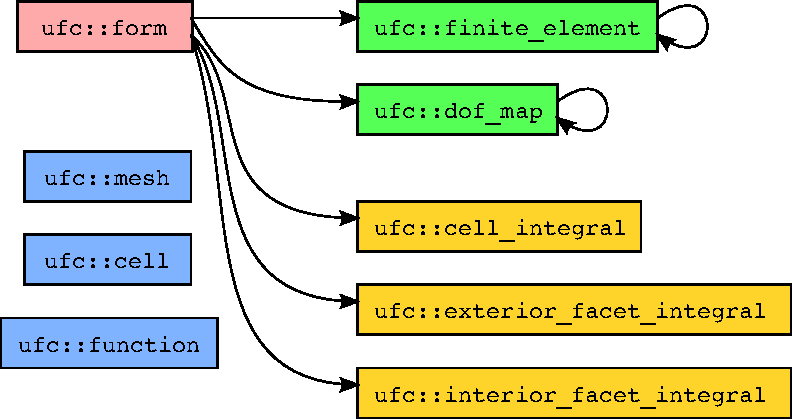
\includegraphics[width=\largefig]{chapters/alnes-2/pdf/ufc_classes.pdf}
  \caption{Schematic overview of some of the UFC classes. Arrows indicate dependencies.}
  \label{fig:uml}
\end{figure}

The UFC interface\footnote{This chapter describes version 1.4 of the
  UFC interface.} consists of a small collection of abstract C++
classes that represent common components for assembling tensors using
the finite element method. The full UFC interface is specified in a
single header file~\emp{ufc.h}. The UFC classes are accompanied by a
set of conventions for numbering of cell data and other arrays. Data
is passed as plain C arrays for efficiency and minimal dependencies.
Most functions are declared \emp{const}, reflecting that the
operations they represent should not change the outcome of future
operations.\footnote{The exceptions are the functions to initialize a
  \emp{dofmap}.}

\subsection{Class relations}

Figure (\ref{fig:uml}) shows all UFC classes and their relations. The
classes \emp{mesh}, \emp{cell}, and \emp{function} provide the means
for communicating mesh and coefficient function data as arguments.
The integrals of~\eqref{eq:form_integrals} are represented by one of
the following classes:
\begin{itemize}
\item
  \emp{cell\_integral},
\item
  \emp{exterior\_facet\-\_inte\-gral},
\item
  \emp{interior\_facet\-\_inte\-gral}.
\end{itemize}
Subclasses of \emp{form} must implement factory functions which may be
called to create integral objects. These objects in turn know how to
compute their respective contribution from a cell or facet during
assembly. A code fragment from the \emp{form} class declaration is
shown below.

\begin{c++}
class form
{
public:

  ...

  /// Create a new cell integral on sub domain i
  virtual cell_integral* create_cell_integral(unsigned int i) const = 0;

  /// Create a new exterior facet integral on sub domain i
  virtual exterior_facet_integral*
  create_exterior_facet_integral(unsigned int i) const = 0;

  /// Create a new interior facet integral on sub domain i
  virtual interior_facet_integral*
  create_interior_facet_integral(unsigned int i) const = 0;

};
\end{c++}

The \emp{form} class also specifies functions for creating
\emp{finite\_element} and \emp{dofmap} objects for the finite
element function spaces $\{V_{j,h}\}_{j=1}^{\rho}$ and
$\{W_{j,h}\}_{j=1}^n$ of the variational form. The
\emp{finite\_element} object provides functionality such as evaluation
of degrees of freedom and evaluation of basis functions and their
derivatives. The \emp{dofmap} object provides functionality such as
tabulating the local-to-global map of degrees of freedom on a single
element, as well as tabulation of subsets associated with particular
mesh entities, which is used to apply Dirichlet boundary conditions
and build connectivity information.

Both the \emp{finite\_element} and \emp{dofmap} classes can
represent mixed elements, in which case it is possible to obtain
\emp{finite\_element} and \emp{dofmap} objects for each subelement
in a hierarchical manner. Vector elements composed of scalar elements
are in this context seen as special cases of mixed elements where all
subelements are equal. As an example, consider the \emp{dofmap} for
a $\mathcal{P}_2$--$\mathcal{P}_1$ Taylor--Hood element. From this
\emp{dofmap} it is possible to extract one \emp{dofmap} for the
quadratic vector element and one \emp{dofmap} for the linear scalar
element. From the vector element, a \emp{dofmap} for the quadratic
scalar element of each vector component can be obtained. This can be
used to access subcomponents from the solution of a mixed system.

\subsection{Stages in the assembly algorithm}

Next, we focus on a few key parts of the interface and explain how
these can be used to implement the assembly algorithm presented in
Chapter~\ref{chap:logg-3}. The general algorithm consists of three
stages: (i) assembling the contributions from all cells, (ii)
assembling the contributions from all exterior facets, and (iii)
assembling the contributions from all interior facets.

Each of the three assembly stages (i)--(iii) is further composed of
five steps. In the first step, a cell~$T$ is fetched from the mesh,
typically implemented by filling a \emp{cell} structure (see
Figure~\ref{fig:cellcode}) with coordinate data and global numbering
of the mesh entities in the cell. This step depends on the specific
mesh being used.

\begin{figure}
\begin{c++}
class cell
{
public:

  /// Constructor
  cell(): cell_shape(interval),
          topological_dimension(0), geometric_dimension(0),
          entity_indices(0), coordinates(0) {}

  /// Destructor
  virtual ~cell() {}

  /// Shape of the cell
  shape cell_shape;

  /// Topological dimension of the mesh
  unsigned int topological_dimension;

  /// Geometric dimension of the mesh
  unsigned int geometric_dimension;

  /// Array of global indices for the mesh entities of the cell
  unsigned int** entity_indices;

  /// Array of coordinates for the vertices of the cell
  double** coordinates;

  /// Cell index (short-cut for entity_indices[topological_dimension][0])
  unsigned int index;

  /// Local facet index
  int local_facet;

  /// Unique mesh identifier
  int mesh_identifier;

};
\end{c++}
\caption{Data structure for communicating cell data.}
\label{fig:cellcode}
\end{figure}

In the second step, the coefficients in $\{W_{j,h}\}_{j=1}^n$ are
restricted to the local cell~$T$. If a coefficient $w_j$ is not given
as a linear combination of basis functions for $W_{j,h}$, it must at
this step be interpolated into $W_{j,h}$, using the interpolant
defined by the degrees of freedom of $W_{j,h}$. One common choice of
interpolation is point evaluation at the set of nodal points. In this
case, the coefficient function is passed as an implementation of the
\emp{function} interface (a simple functor) to the
function~\emp{evaluate\_dofs} in the UFC \emp{finite\_element} class.

\begin{c++}
/// Evaluate linear functionals for all dofs on the function f
virtual void evaluate_dofs(double* values,
                           const function& f,
                           const cell& c) const = 0;
\end{c++}
Here, \emp{double* values} is a pointer to the first element of an
array of double precision floating point numbers which will be filled
with the values of the degrees of freedom of the function~\emp{f} on
the current cell.

In the third step, the local-to-global map of degrees of freedom is
tabulated for each of the function spaces. That is, for each of the
local discrete finite element spaces on $T$, we tabulate the
corresponding global degrees of freedom.

\begin{c++}
/// Tabulate the local-to-global mapping of dofs on a cell
void dofmap::tabulate_dofs(unsigned int* dofs,
                           const mesh& m,
                           const cell& c) const
\end{c++}
Here, \emp{unsigned int* dofs} is a pointer to the first element of an
array of unsigned integers that will be filled with the
local-to-global map on the current cell during the function call.

In the fourth step, the local element tensor contribution (cell or
exterior/interior facet tensor) is computed. This is done by a call to
the function~\emp{tabulate\_tensor}, illustrated below for a cell
integral.
\begin{c++}
/// Tabulate the tensor for the contribution from a local cell
virtual void tabulate_tensor(double* A,
                             const double * const * w,
                             const cell& c) const = 0;
\end{c++}
Here, \emp{double* A} is a pointer to the first element of an array of
double precision floating point numbers which will be filled with the
values of the element tensor, flattened into one array of
numbers. Similarly, one may evaluate interior and exterior facet
contributions using slightly different function signatures.

Finally, at the fifth step, the local element tensor contributions are
added to the global tensor, using the local-to-global maps previously
obtained by calls to the \emp{tabulate\_dofs} function. This is an
operation that depends on the linear algebra backend used to store the
global tensor.

\subsection{Code generation utilities}

UFC provides a number of utilities that can be used by form compilers
to simplify the code generation process, including templates for
creating subclasses of UFC classes and utilities for just-in-time
compilation.  These are distributed as part of the \emp{ufc\_utils}
Python module.

Templates are available for all UFC classes listed in
Figure~\ref{fig:uml} and consist of format strings for the skeleton of
each subclass. The following code illustrates how to generate a
subclass of the UFC \emp{form} class.

\begin{c++}
from ufc_utils import form_combined

implementation = {}
implementation["classname"] = "my_form"
implementation["members"] = ""
implementation["constructor_arguments"] = ""
implementation["initializer_list"] = ""
implementation["constructor"] = "// Do nothing"
implementation["destructor"] = "// Do nothing"
implementation["signature"] = "return \"my form\""
implementation["rank"] = "return 2;"
implementation["num_coefficients"] = "return 0;"
implementation["num_cell_domains"] = "return 3;"
implementation["num_interior_facet_domains"] = "return 1;"
implementation["num_exterior_facet_domains"] = "return 0;"
implementation["create_finite_element"] = "\
switch (i)
{
case 0:
  return new my_finite_element_0();
case 1:
  return new my_finite_element_1();
default:
  return 0;
}"
implementation["create_dofmap"] = "\
switch (i)
{
case 0:
  return new my_dofmap_0();
case 1:
  return new my_dofmap_1();
default:
  return 0;
}"
implementation["create_cell_integral"] = "\
switch (i)
{
case 0:
  return new my_cell_integral_0();
case 1:
  return new my_cell_integral_1();
case 2:
  return new my_cell_integral_2();
default:
  return 0;
}"
implementation["create_exterior_facet_integral"] = "\
return new my_exterior_facet_integral();"
implementation["create_interior_facet_integral"] = "return 0;"

print form_combined % implementation
\end{c++}

This generates code for a single header file that also contains the
implementation of each function in the UFC \emp{form} interface. It is
also possible to generate code for separate header (\emp{.h}) and
implementation (\emp{.cpp}) files by using the \emp{form\_header} and
\emp{form\_implementation} templates.

The \emp{ufc\_utils} module also contains the utility function
\emp{build\_ufc\_module} that can be called to build a Python module
based on generated UFC code. This process involves compilation,
linking, and loading of the generated C++ code as well as generating a
Python wrapper module using Instant/SWIG as described in
Chapter~\ref{chap:wilbers}.

%------------------------------------------------------------------------------
\section{Examples}
\label{sec:alnes-2:examples}

In this section, we demonstrate how UFC can be used in practice for
assembly of finite element forms. First, we demonstrate how one may
implement a simple assembler based on generated UFC code. We then show
examples of input to the form compilers FFC and SFC as well as part of
the corresponding UFC code generated as output.

\subsection{Assembler}

The simple assembler presented in this section assumes that the
degrees of freedom of the finite element spaces involved depend only
on vertices; that is, we assume piecewise linear elements. We also
assume that the assembled form is a tensor of rank two (a matrix),
that we may insert values into the given matrix data structure by
simply assigning values to the entries of the matrix, that the form
does not depend on any coefficients, and that the form is expressed as
a single cell integral. In practice, the efficient insertion of
entries into a sparse matrix typically requires a the use of a special
optimized library call. For example, entries may be inserted (added)
to a sparse PETSc matrix by a call to \emp{MatSetValues} and to a
sparse Trilinos/Epetra matrix by a call to
\emp{SumIntoGlobalValues}. For a complete implementation of an
assembler for general rank tensors and generic linear algebra
libraries that provide an insertion operation, we refer to the class
\emp{Assembler} in DOLFIN (\emp{Assembler.cpp}). The code example
presented below is available in the supplementary material for this
chapter (\emp{assemble.cpp}).

\begin{c++}
void assemble(Matrix& A, ufc::form& form, dolfin::Mesh& mesh)
{
  // Get dimensions
  const uint D = mesh.topology().dim();
  const uint d = mesh.geometry().dim();

  // Initialize UFC mesh data structure
  ufc::mesh ufc_mesh;
  ufc_mesh.topological_dimension = D;
  ufc_mesh.geometric_dimension = d;
  ufc_mesh.num_entities = new uint[D + 1];
  for (uint i = 0; i <= D; i++)
    ufc_mesh.num_entities[i] = 0;
  ufc_mesh.num_entities[0] = mesh.num_vertices();
  ufc_mesh.num_entities[D] = mesh.num_cells();

  // Initialize UFC cell data structure, assuming that the
  // cell is a simplex and only vertices are used for dofs
  ufc::cell ufc_cell;
  switch (D)
  {
  case 1:
    ufc_cell.cell_shape = ufc::interval;
    break;
  case 2:
    ufc_cell.cell_shape = ufc::triangle;
    break;
  default:
    ufc_cell.cell_shape = ufc::tetrahedron;
    break;
  }
  ufc_cell.topological_dimension = D;
  ufc_cell.geometric_dimension = d;
  ufc_cell.entity_indices = new uint * [D + 1];
  for (uint i = 0; i <= D; i++)
    ufc_cell.entity_indices[i] = 0;
  uint vertices_per_cell = D + 1;
  ufc_cell.entity_indices[0] = new uint[vertices_per_cell];
  ufc_cell.entity_indices[D] = new uint[1];
  ufc_cell.coordinates = new double * [vertices_per_cell];
  for (uint i = 0; i <= D; i++)
    ufc_cell.coordinates[i] = new double[d];

  // Create cell integrals, assuming there is only one
  ufc::cell_integral* cell_integral = form.create_cell_integral(0);

  // Create dofmaps for rows and columns
  ufc::dofmap* dofmap_0 = form.create_dofmap(0);
  ufc::dofmap* dofmap_1 = form.create_dofmap(1);

  // Initialize dofmaps
  dofmap_0->init_mesh(ufc_mesh);
  dofmap_1->init_mesh(ufc_mesh);

  // Omitting code for dofmap initialization on cells, which is not
  // needed for code generated by FFC but which is generally required

  // Get local and global dimensions
  uint m = dofmap_0->max_local_dimension();
  uint n = dofmap_1->max_local_dimension();
  uint M = dofmap_0->global_dimension();
  uint N = dofmap_1->global_dimension();

  // Initialize array of local-to-global maps
  uint* dofs_0 = new uint[m];
  uint* dofs_1 = new uint[n];

  // Initialize array of values for the cell matrix
  double* A_T = new double[m * n];

  // Initialize global matrix
  A.init(M, N);

  // Iterate over the cells of the mesh
  for (dolfin::CellIterator cell(mesh); !cell.end(); ++cell)
  {
    // Update UFC cell data structure for current cell
    ufc_cell.entity_indices[D][0] = cell->index();
    for (dolfin::VertexIterator vertex(*cell); !vertex.end(); ++vertex)
    {
      ufc_cell.entity_indices[0][vertex.pos()] = vertex->index();
      for (uint i = 0; i < d; i++)
        ufc_cell.coordinates[vertex.pos()][i] = vertex->x(i);
    }

    // Compute local-to-global map for degrees of freedom
    dofmap_0->tabulate_dofs(dofs_0, ufc_mesh, ufc_cell);
    dofmap_1->tabulate_dofs(dofs_1, ufc_mesh, ufc_cell);

    // Compute the cell matrix A_T
    cell_integral->tabulate_tensor(A_T, 0, ufc_cell);

    // Add entries to global matrix
    for (uint i = 0; i < m; i++)
      for (uint j = 0; j < m; j++)
        A(dofs_0[i], dofs_1[j]) += A_T[i*n + j];
  }

  // Omitting code for deleting allocated arrays
}
\end{c++}

\subsection{Generated UFC code}

The form language UFL described in Chapter~\ref{chap:alnes-1} provides
a simple language for specification of variational forms, which may be
entered either directly in Python or in text files given to a form
compiler.  We consider the following definition of the bilinear form
$a(u, v) = \inner{\nabla u}{\nabla v}$ in UFL:
\begin{c++}
element = FiniteElement("Lagrange", "triangle", 1)

u = TrialFunction(element)
v = TestFunction(element)

a = inner(grad(u), grad(v))*dx
\end{c++}

When compiling this code, a C++ header file is created, containing UFC
code that may be used to assemble the global sparse stiffness matrix
for Poisson's equation. Below, we present the code generated for
evaluation of the element stiffness matrix for the bilinear
form~\emp{a} using FFC. Similar code may be generated using SFC.

\begin{c++}
/// Tabulate the tensor for the contribution from a local cell
virtual void tabulate_tensor(double* A,
                             const double * const * w,
                             const ufc::cell& c) const
{
  // Number of operations (multiply-add pairs) for Jacobian data:      11
  // Number of operations (multiply-add pairs) for geometry tensor:    8
  // Number of operations (multiply-add pairs) for tensor contraction: 11
  // Total number of operations (multiply-add pairs):                  30

  // Extract vertex coordinates
  const double * const * x = c.coordinates;

  // Compute Jacobian of affine map from reference cell
  const double J_00 = x[1][0] - x[0][0];
  const double J_01 = x[2][0] - x[0][0];
  const double J_10 = x[1][1] - x[0][1];
  const double J_11 = x[2][1] - x[0][1];

  // Compute determinant of Jacobian
  double detJ = J_00*J_11 - J_01*J_10;

  // Compute inverse of Jacobian
  const double K_00 =  J_11 / detJ;
  const double K_01 = -J_01 / detJ;
  const double K_10 = -J_10 / detJ;
  const double K_11 =  J_00 / detJ;

  // Set scale factor
  const double det = std::abs(detJ);

  // Compute geometry tensor
  const double G0_0_0 = det*(K_00*K_00 + K_01*K_01);
  const double G0_0_1 = det*(K_00*K_10 + K_01*K_11);
  const double G0_1_0 = det*(K_10*K_00 + K_11*K_01);
  const double G0_1_1 = det*(K_10*K_10 + K_11*K_11);

  // Compute element tensor
  A[0] = 0.500000000000000*G0_0_0 + 0.500000000000000*G0_0_1
       + 0.500000000000000*G0_1_0 + 0.500000000000000*G0_1_1;
  A[1] = -0.500000000000000*G0_0_0 - 0.500000000000000*G0_1_0;
  A[2] = -0.500000000000000*G0_0_1 - 0.500000000000000*G0_1_1;
  A[3] = -0.500000000000000*G0_0_0 - 0.500000000000000*G0_0_1;
  A[4] = 0.500000000000000*G0_0_0;
  A[5] = 0.500000000000000*G0_0_1;
  A[6] = -0.500000000000000*G0_1_0 - 0.500000000000000*G0_1_1;
  A[7] = 0.500000000000000*G0_1_0;
  A[8] = 0.500000000000000*G0_1_1;
}
\end{c++}

Having computed the element tensor, one needs to compute the
local-to-global map in order to know where to insert the local
contributions in the global tensor. This map may be obtained by
calling the member function \emp{tabulate\_dofs} of the class
\emp{dofmap}. FFC uses an implicit ordering scheme, based on the
indices of the topological entities in the mesh. This information may
be extracted from the \emp{cell} attribute \emp{entity\_indices}.  For
linear Lagrange elements on triangles, each degree of freedom is
associated with a global vertex. Hence, FFC constructs the map by
picking the corresponding global vertex number for each degree of
freedom as demonstrated below.
\begin{c++}
virtual void tabulate_dofs(unsigned int* dofs,
                           const ufc::mesh& m,
                           const ufc::cell& c) const
{
  dofs[0] = c.entity_indices[0][0];
  dofs[1] = c.entity_indices[0][1];
  dofs[2] = c.entity_indices[0][2];
}
\end{c++}

For quadratic Lagrange elements, a similar map is generated based on
global vertex and edge numbers (entities of dimension zero and one
respectively). We list the code for \emp{tabulate\_dofs} generated by
FFC for quadratic Lagrange elements below.
\begin{c++}
virtual void tabulate_dofs(unsigned int* dofs,
                           const ufc::mesh& m,
                           const ufc::cell& c) const
{
  unsigned int offset = 0;
  dofs[0] = offset + c.entity_indices[0][0];
  dofs[1] = offset + c.entity_indices[0][1];
  dofs[2] = offset + c.entity_indices[0][2];
  offset += m.num_entities[0];
  dofs[3] = offset + c.entity_indices[1][0];
  dofs[4] = offset + c.entity_indices[1][1];
  dofs[5] = offset + c.entity_indices[1][2];
  offset += m.num_entities[1];
}
\end{c++}

%------------------------------------------------------------------------------
\section{Numbering conventions}
\label{sec:alnes-2:numbering}

UFC relies on a set of numbering conventions for cells, vertices and
other mesh entities. The numbering scheme ensures that form compilers
(FFC and SFC) and assemblers (DOLFIN) can communicate data required
for tabulating the cell and facet tensors as well as local-to-global
maps.

\subsection{Reference cells}

\index{reference cells}

The following five reference cells are covered by the UFC specification:
the reference \emph{interval},
the reference \emph{triangle},
the reference \emph{quadrilateral},
the reference \emph{tetrahedron}, and
the reference \emph{hexahedron} (see Table~\ref{tab:ufc_reference_cells}).
The UFC specification assumes that each cell in a finite element mesh
is always isomorphic to one of the reference cells.

\begin{table}
\linespread{1.2}\selectfont
  \begin{center}
    \begin{tabular}{|l|c|c|c|}
      \hline
      Reference cell & Dimension & \#Vertices & \#Facets \\
      \hline
      \hline
      The reference interval      & 1 & 2 & 2 \\
      \hline
      The reference triangle      & 2 & 3 & 3 \\
      \hline
      The reference quadrilateral & 2 & 4 & 4 \\
      \hline
      The reference tetrahedron   & 3 & 4 & 4 \\
      \hline
      The reference hexahedron    & 3 & 8 & 6 \\
      \hline
    \end{tabular}
    \caption{Reference cells covered by the UFC specification.}
    \label{tab:ufc_reference_cells}
  \end{center}
\end{table}

\subsubsection{The reference interval}
\index{interval}

The reference interval is shown in Figure~\ref{fig:interval} and is
defined by its two vertices with coordinates as specified in
Table~\ref{tab:interval,vertices}.

\begin{figure}
  \begin{center}
    \psfrag{0}{$0$}
    \psfrag{1}{$1$}
    \includegraphics[width=10cm]{chapters/alnes-2/eps/interval.eps}
    \caption{The reference interval.}
    \label{fig:interval}
  \end{center}
\end{figure}

\begin{table}
\linespread{1.2}\selectfont
  \begin{center}
    \begin{tabular}{|c|c|}
      \hline
      Vertex & Coordinate \\
      \hline
      \hline
      $v_0$ & $x = 0$ \\
      \hline
      $v_1$ & $x = 1$ \\
      \hline
    \end{tabular}
    \caption{Vertex coordinates of the reference interval.}
    \label{tab:interval,vertices}
  \end{center}
\end{table}

\subsubsection{The reference triangle}
\index{triangle}

The reference triangle is shown in Figure~\ref{fig:triangle} and is
defined by its three vertices with coordinates as specified in
Table~\ref{tab:triangle,vertices}.

\begin{figure}
  \begin{center}
    \psfrag{v0}{$(0, 0)$}
    \psfrag{v1}{$(1, 0)$}
    \psfrag{v2}{$(0, 1)$}
    \includegraphics[width=8cm]{chapters/alnes-2/eps/triangle.eps}
    \caption{The reference triangle.}
    \label{fig:triangle}
  \end{center}
\end{figure}

\begin{table}
\linespread{1.2}\selectfont
  \begin{center}
    \begin{tabular}{|c|c|}
      \hline
      Vertex & Coordinate \\
      \hline
      \hline
      $v_0$ & $x = (0, 0)$ \\
      \hline
      $v_1$ & $x = (1, 0)$ \\
      \hline
      $v_2$ & $x = (0, 1)$ \\
      \hline
    \end{tabular}
    \caption{Vertex coordinates of the reference triangle.}
    \label{tab:triangle,vertices}
  \end{center}
\end{table}

\subsubsection{The reference quadrilateral}
\index{quadrilateral}

The reference quadrilateral is shown in Figure~\ref{fig:quadrilateral}
and is defined by its four vertices with coordinates as specified in
Table~\ref{tab:quadrilateral,vertices}.

\begin{figure}
  \begin{center}
    \psfrag{v0}{$(0, 0)$}
    \psfrag{v1}{$(1, 0)$}
    \psfrag{v2}{$(1, 1)$}
    \psfrag{v3}{$(0, 1)$}
    \includegraphics[width=8cm]{chapters/alnes-2/eps/quadrilateral.eps}
    \caption{The reference quadrilateral.}
    \label{fig:quadrilateral}
  \end{center}
\end{figure}

\begin{table}
\linespread{1.2}\selectfont
  \begin{center}
    \begin{tabular}{|c|c|}
      \hline
      Vertex & Coordinate \\
      \hline
      \hline
      $v_0$ & $x = (0, 0)$ \\
      \hline
      $v_1$ & $x = (1, 0)$ \\
      \hline
      $v_2$ & $x = (1, 1)$ \\
      \hline
      $v_3$ & $x = (0, 1)$ \\
      \hline
    \end{tabular}
    \caption{Vertex coordinates of the reference quadrilateral.}
    \label{tab:quadrilateral,vertices}
  \end{center}
\end{table}

\subsubsection{The reference tetrahedron}
\index{tetrahedron}

The reference tetrahedron is shown in Figure~\ref{fig:tetrahedron} and
is defined by its four vertices with coordinates as specified in
Table~\ref{tab:tetrahedron,vertices}.

\begin{figure}
  \begin{center}
    \psfrag{v0}{$(0, 0, 0)$}
    \psfrag{v1}{$(1, 0, 0)$}
    \psfrag{v2}{$(0, 1, 0)$}
    \psfrag{v3}{$(0, 0, 1)$}
    \includegraphics[width=6cm]{chapters/alnes-2/eps/tetrahedron.eps}
    \caption{The reference tetrahedron.}
    \label{fig:tetrahedron}
  \end{center}
\end{figure}

\begin{table}
\linespread{1.2}\selectfont
  \begin{center}
    \begin{tabular}{|c|c|}
      \hline
      Vertex & Coordinate \\
      \hline
      \hline
      $v_0$ & $x = (0, 0, 0)$ \\
      \hline
      $v_1$ & $x = (1, 0, 0)$ \\
      \hline
      $v_2$ & $x = (0, 1, 0)$ \\
      \hline
      $v_3$ & $x = (0, 0, 1)$ \\
      \hline
    \end{tabular}
    \caption{Vertex coordinates of the reference tetrahedron.}
    \label{tab:tetrahedron,vertices}
  \end{center}
\end{table}

\subsubsection{The reference hexahedron}
\index{hexahedron}

The reference hexahedron is shown in Figure~\ref{fig:hexahedron} and
is defined by its eight vertices with coordinates as specified in
Table~\ref{tab:hexahedron,vertices}.

\begin{figure}
\linespread{1.2}\selectfont
  \begin{center}
    \psfrag{v0}{$(0, 0, 0)$}
    \psfrag{v1}{$(1, 0, 0)$}
    \psfrag{v2}{$(1, 1, 0)$}
    \psfrag{v3}{$(0, 1, 0)$}
    \psfrag{v4}{$(0, 0, 1)$}
    \psfrag{v5}{$(1, 0, 1)$}
    \psfrag{v6}{$(1, 1, 1)$}
    \psfrag{v7}{$(0, 1, 1)$}
    \includegraphics[width=9cm]{chapters/alnes-2/eps/hexahedron.eps}
    \caption{The reference hexahedron.}
    \label{fig:hexahedron}
  \end{center}
\end{figure}

\begin{table}
\linespread{1.2}\selectfont
  \begin{center}
    \begin{tabular}{|c|c|}
      \hline
      Vertex & Coordinate \\
      \hline
      \hline
      $v_0$ & $x = (0, 0, 0)$ \\
      \hline
      $v_1$ & $x = (1, 0, 0)$ \\
      \hline
      $v_2$ & $x = (1, 1, 0)$ \\
      \hline
      $v_3$ & $x = (0, 1, 0)$ \\
      \hline
    \end{tabular}
    \begin{tabular}{|c|c|}
      \hline
      Vertex & Coordinate \\
      \hline
      \hline
      $v_4$ & $x = (0, 0, 1)$ \\
      \hline
      $v_5$ & $x = (1, 0, 1)$ \\
      \hline
      $v_6$ & $x = (1, 1, 1)$ \\
      \hline
      $v_7$ & $x = (0, 1, 1)$ \\
      \hline
    \end{tabular}
    \caption{Vertex coordinates of the reference hexahedron.}
    \label{tab:hexahedron,vertices}
  \end{center}
\end{table}


\subsection{Numbering of mesh entities}

\index{numbering}

The UFC specification dictates a certain numbering of the vertices,
edges etc. of the cells of a finite element mesh. First, an \emph{ad
hoc} numbering may be picked for the vertices of each cell. Then, the
remaining entities are ordered based on a simple rule, as described in
detail below.

\paragraph{Basic concepts}
\index{mesh entity}
\index{topological dimension}

The topological entities of a cell (or mesh) are referred to as
\emph{mesh entities}. A mesh entity can be identified by a pair $(d,
i)$, where $d$ is the topological dimension of the mesh entity and $i$
is a unique index of the mesh entity. Mesh entities are numbered
within each topological dimension from $0$ to $n_d-1$, where $n_d$ is
the number of mesh entities of topological dimension $d$.

For convenience, mesh entities of topological dimension~$0$ are
referred to as \emph{vertices}, entities of dimension~$1$ as
\emph{edges}, entities of dimension~$2$ as \emph{faces}, entities of
\emph{codimension}~$1$ as \emph{facets}, and entities of codimension~$0$
as \emph{cells}. These concepts are summarized in the table below.

\vspace{0.5cm}
\begin{center}
  \begin{tabular}{lcc} \toprule Entity & Dimension &
    Codimension \\ \hline Vertex & $0$ & -- \\ Edge & $1$ & -- \\ Face
    & $2$ & -- \\ & & \\ Facet & -- & $1$ \\ Cell & -- &
    $0$ \\ \bottomrule \end{tabular}
\end{center}
\vspace{0.5cm}

Thus, the vertices of a tetrahedron are identified as $v_0 = (0, 0)$,
$v_1 = (0, 1)$, $v_2 = (0, 2)$ and $v_3 = (0, 3)$, the edges are $e_0
= (1, 0)$, $e_1 = (1, 1)$, $e_2 = (1, 2)$, $e_3 = (1, 3)$, $e_4 = (1,
4)$ and $e_5 = (1, 5)$, the faces (facets) are $f_0 = (2, 0)$, $f_1 =
(2, 1)$, $f_2 = (2, 2)$ and $f_3 = (2, 3)$, and the cell itself is
$c_0 = (3, 0)$.

\paragraph{Numbering of vertices.}
\index{vertex numbering}

For simplicial cells (intervals, triangles and tetrahedra) of a finite
element mesh, the vertices are numbered locally based on the
corresponding global vertex numbers. In particular, a tuple of
increasing local vertex numbers corresponds to a tuple of increasing
global vertex numbers. This is illustrated in
Figure~\ref{fig:numbering_example_triangles} for a mesh consisting of
two triangles.

\begin{figure}[htbp]
  \begin{center}
    \fenicsfig{alnes-2}{numbering_example_triangles}{\largefig}
    \caption{The vertices of a simplicial mesh are numbered locally
      based on the corresponding global vertex numbers.}
    \label{fig:numbering_example_triangles}
  \end{center}
\end{figure}

For non-simplicial cells (quadrilaterals and hexahedra), the numbering
is arbitrary, as long as each cell is topologically isomorphic to the corresponding
reference cell by matching each vertex with the corresponding vertex
in the reference cell. This is illustrated in
Figure~\ref{fig:numbering_example_quadrilaterals} for a mesh
consisting of two quadrilaterals.

\begin{figure}
  \begin{center}
    \fenicsfig{alnes-2}{numbering_example_quadrilaterals}{\largefig}
    \caption{The local numbering of vertices of a non-simplicial mesh
      is arbitrary, as long as each cell is topologically isomorphic
      to the reference cell by matching each vertex to the
      corresponding vertex of the reference cell.}
    \label{fig:numbering_example_quadrilaterals}
  \end{center}
\end{figure}

\paragraph{Numbering of other mesh entities.}

When the vertices have been numbered, the remaining mesh entities are
numbered within each topological dimension based on a
\emph{lexicographical ordering} of the corresponding ordered tuples of
\emph{non-incident vertices}.

As an illustration, consider the numbering of edges (the mesh entities
of topological dimension one) on the reference triangle in
Figure~\ref{fig:orderingexample,triangle}. To number the edges of the
reference triangle, we identify for each edge the corresponding
non-incident vertices. For each edge, there is only one such vertex
(the vertex opposite to the edge). We thus identify the three edges in
the reference triangle with the tuples $(v_0)$, $(v_1)$, and $(v_2)$. The
first of these is edge $e_0$ between vertices $v_1$ and $v_2$ opposite
to vertex $v_0$, the second is edge $e_1$ between vertices $v_0$ and
$v_2$ opposite to vertex $v_1$, and the third is edge $e_2$ between
vertices $v_0$ and $v_1$ opposite to vertex $v_2$.

Similarly, we identify the six edges of the reference tetrahedron with
the corresponding non-incident tuples $(v_0, v_1)$, $(v_0, v_2)$,
$(v_0, v_3)$, $(v_1, v_2)$, $(v_1, v_3)$ and $(v_2, v_3)$. The first
of these is edge $e_0$ between vertices $v_2$ and $v_3$ opposite to
vertices $v_0$ and $v_1$ as shown in
Figure~\ref{fig:orderingexample,tetrahedron}.

\begin{figure}
  \begin{center}
    \fenicsfig{alnes-2}{ordering_example_triangle}{\smallfig}
    \caption{Mesh entities are ordered based on a lexicographical
      ordering of the corresponding ordered tuples of non-incident
      vertices. The first edge $e_0$ is non-incident to vertex $v_0$.}
    \label{fig:orderingexample,triangle}
  \end{center}
\end{figure}

\begin{figure}
  \begin{center}
    \fenicsfig{alnes-2}{ordering_example_tetrahedron}{\smallfig}
    \caption{Mesh entities are ordered based on a lexicographical
      ordering of the corresponding ordered tuples of non-incident
      vertices. The first edge $e_0$ is non-incident to vertices $v_0$
      and $v_1$.}
    \label{fig:orderingexample,tetrahedron}
  \end{center}
\end{figure}

\paragraph{Relative ordering.}

The relative ordering of mesh entities with respect to other incident
mesh entities follows by sorting the entities by their (global)
indices. Thus, the pair of vertices incident to the first edge $e_0$
of a triangular cell is $(v_1, v_2)$, not $(v_2, v_1)$. Similarly, the
first face $f_0$ of a tetrahedral cell is incident to vertices $(v_1,
v_2, v_3)$.

For simplicial cells, the relative ordering in combination with the
convention of numbering the vertices locally based on global vertex
indices means that two incident cells will always agree on the
orientation of incident subsimplices. Thus, two incident triangles
will agree on the orientation of the common edge and two incident
tetrahedra will agree on the orientation of the common edge(s) and the
orientation of the common face (if any). This is illustrated in
Figure~\ref{fig:orientation_example_triangles} for two incident
triangles sharing a common edge. This leads to practical advantages in
the assembly of higher-order, $\Hdiv$ and $\Hcurl$ elements.

\begin{figure}[htbp]
  \begin{center}
    \fenicsfig{alnes-2}{orientation_example_triangles}{\largefig}
    \caption{Two incident triangles will always agree on the
      orientation of the common edge.}
    \label{fig:orientation_example_triangles}
  \end{center}
\end{figure}

\paragraph{Limitations.}

The UFC specification is only concerned with the ordering of mesh
entities with respect to entities of larger topological dimension. In
other words, the UFC specification is only concerned with the ordering
of incidence relations of the class $d - d'$ where $d > d'$. For
example, the UFC specification is not concerned with the ordering of
incidence relations of the class $0 - 1$, that is, the ordering of
edges incident to vertices.

\paragraph{Numbering of mesh entities on intervals.}
\index{interval}

The numbering of mesh entities on interval cells is summarized in the
table below.

\begin{center}
  \begin{tabular}{ccc}
    \toprule
    Entity & Incident vertices & Non-incident vertices \\
    \hline
    $v_0 = (0, 0)$ & $(v_0)$ & $(v_1)$ \\
    $v_1 = (0, 1)$ & $(v_1)$ & $(v_0)$ \\
    $c_0 = (1, 0)$ & $(v_0, v_1)$ & $\emptyset$ \\
    \bottomrule
  \end{tabular}
\end{center}

\paragraph{Numbering of mesh entities on triangular cells.}
\index{triangle}

The numbering of mesh entities on triangular cells is summarized in the
table below.

\begin{center}
  \begin{tabular}{ccc}
    \toprule
    Entity & Incident vertices & Non-incident vertices \\
    \hline
    $v_0 = (0, 0)$ & $(v_0)$ & $(v_1, v_2)$ \\
    $v_1 = (0, 1)$ & $(v_1)$ & $(v_0, v_2)$ \\
    $v_2 = (0, 2)$ & $(v_2)$ & $(v_0, v_1)$ \\
    $e_0 = (1, 0)$ & $(v_1, v_2)$ & $(v_0)$ \\
    $e_1 = (1, 1)$ & $(v_0, v_2)$ & $(v_1)$ \\
    $e_2 = (1, 2)$ & $(v_0, v_1)$ & $(v_2)$ \\
    $c_0 = (2, 0)$ & $(v_0, v_1, v_2)$ & $\emptyset$ \\
    \bottomrule
  \end{tabular}
\end{center}

\paragraph{Numbering of mesh entities on quadrilateral cells.}
\index{quadrilateral}

The numbering of mesh entities on quadrilateral cells is summarized in the
table below.

\begin{center}
  \begin{tabular}{ccc}
    \toprule
    Entity & Incident vertices & Non-incident vertices \\
    \hline
    $v_0 = (0, 0)$ & $(v_0)$ & $(v_1, v_2, v_3)$ \\
    $v_1 = (0, 1)$ & $(v_1)$ & $(v_0, v_2, v_3)$ \\
    $v_2 = (0, 2)$ & $(v_2)$ & $(v_0, v_1, v_3)$ \\
    $v_3 = (0, 3)$ & $(v_3)$ & $(v_0, v_1, v_2)$ \\
    $e_0 = (1, 0)$ & $(v_2, v_3)$ & $(v_0, v_1)$ \\
    $e_1 = (1, 1)$ & $(v_1, v_2)$ & $(v_0, v_3)$ \\
    $e_2 = (1, 2)$ & $(v_0, v_3)$ & $(v_1, v_2)$ \\
    $e_3 = (1, 3)$ & $(v_0, v_1)$ & $(v_2, v_3)$ \\
    $c_0 = (2, 0)$ & $(v_0, v_1, v_2, v_3)$ & $\emptyset$ \\
    \bottomrule
  \end{tabular}
\end{center}

\paragraph{Numbering of mesh entities on tetrahedral cells.}
\index{tetrahedron}

The numbering of mesh entities on tetrahedral cells is summarized in the
table below.

\begin{center}
  \begin{tabular}{ccc}
    \toprule
    Entity & Incident vertices & Non-incident vertices \\
    \hline
    $v_0 = (0, 0)$ & $(v_0)$ & $(v_1, v_2, v_3)$ \\
    $v_1 = (0, 1)$ & $(v_1)$ & $(v_0, v_2, v_3)$ \\
    $v_2 = (0, 2)$ & $(v_2)$ & $(v_0, v_1, v_3)$ \\
    $v_3 = (0, 3)$ & $(v_3)$ & $(v_0, v_1, v_2)$ \\
    $e_0 = (1, 0)$ & $(v_2, v_3)$ & $(v_0, v_1)$ \\
    $e_1 = (1, 1)$ & $(v_1, v_3)$ & $(v_0, v_2)$ \\
    $e_2 = (1, 2)$ & $(v_1, v_2)$ & $(v_0, v_3)$ \\
    $e_3 = (1, 3)$ & $(v_0, v_3)$ & $(v_1, v_2)$ \\
    $e_4 = (1, 4)$ & $(v_0, v_2)$ & $(v_1, v_3)$ \\
    $e_5 = (1, 5)$ & $(v_0, v_1)$ & $(v_2, v_3)$ \\
    $f_0 = (2, 0)$ & $(v_1, v_2, v_3)$ & $(v_0)$ \\
    $f_1 = (2, 1)$ & $(v_0, v_2, v_3)$ & $(v_1)$ \\
    $f_2 = (2, 2)$ & $(v_0, v_1, v_3)$ & $(v_2)$ \\
    $f_3 = (2, 3)$ & $(v_0, v_1, v_2)$ & $(v_3)$ \\
    $c_0 = (3, 0)$ & $(v_0, v_1, v_2, v_3)$ & $\emptyset$ \\
    \bottomrule
  \end{tabular}
\end{center}

\paragraph{Numbering of mesh entities on hexahedral cells.}
\index{hexahedron}

The numbering of mesh entities on hexahedral cells is summarized in
the table below.

\begin{center}
  \begin{tabular}{ccc}
    \toprule
    Entity & Incident vertices & Non-incident vertices \\
    \hline
    $v_0 = (0, 0)$ & $(v_0)$ & $(v_1, v_2, v_3, v_4, v_5, v_6, v_7)$ \\
    $v_1 = (0, 1)$ & $(v_1)$ & $(v_0, v_2, v_3, v_4, v_5, v_6, v_7)$ \\
    $v_2 = (0, 2)$ & $(v_2)$ & $(v_0, v_1, v_3, v_4, v_5, v_6, v_7)$ \\
    $v_3 = (0, 3)$ & $(v_3)$ & $(v_0, v_1, v_2, v_4, v_5, v_6, v_7)$ \\
    $v_4 = (0, 4)$ & $(v_4)$ & $(v_0, v_1, v_2, v_3, v_5, v_6, v_7)$ \\
    $v_5 = (0, 5)$ & $(v_5)$ & $(v_0, v_1, v_2, v_3, v_4, v_6, v_7)$ \\
    $v_6 = (0, 6)$ & $(v_6)$ & $(v_0, v_1, v_2, v_3, v_4, v_5, v_7)$ \\
    $v_7 = (0, 7)$ & $(v_7)$ & $(v_0, v_1, v_2, v_3, v_4, v_5, v_6)$ \\
    $e_0 = (1, 0)$ & $(v_6, v_7)$ & $(v_0, v_1, v_2, v_3, v_4, v_5)$ \\
    $e_1 = (1, 1)$ & $(v_5, v_6)$ & $(v_0, v_1, v_2, v_3, v_4, v_7)$ \\
    $e_2 = (1, 2)$ & $(v_4, v_7)$ & $(v_0, v_1, v_2, v_3, v_5, v_6)$ \\
    $e_3 = (1, 3)$ & $(v_4, v_5)$ & $(v_0, v_1, v_2, v_3, v_6, v_7)$ \\
    $e_4 = (1, 4)$ & $(v_3, v_7)$ & $(v_0, v_1, v_2, v_4, v_5, v_6)$ \\
    $e_5 = (1, 5)$ & $(v_2, v_6)$ & $(v_0, v_1, v_3, v_4, v_5, v_7)$ \\
    $e_6 = (1, 6)$ & $(v_2, v_3)$ & $(v_0, v_1, v_4, v_5, v_6, v_7)$ \\
    $e_7 = (1, 7)$ & $(v_1, v_5)$ & $(v_0, v_2, v_3, v_4, v_6, v_7)$ \\
    $e_8 = (1, 8)$ & $(v_1, v_2)$ & $(v_0, v_3, v_4, v_5, v_6, v_7)$ \\
    $e_9 = (1, 9)$ & $(v_0, v_4)$ & $(v_1, v_2, v_3, v_5, v_6, v_7)$ \\
    $e_{10} = (1, 10)$ & $(v_0, v_3)$ & $(v_1, v_2, v_4, v_5, v_6, v_7)$ \\
    $e_{11} = (1, 11)$ & $(v_0, v_1)$ & $(v_2, v_3, v_4, v_5, v_6, v_7)$ \\
    $f_0 = (2, 0)$ & $(v_4, v_5, v_6, v_7)$ & $(v_0, v_1, v_2, v_3)$ \\
    $f_1 = (2, 1)$ & $(v_2, v_3, v_6, v_7)$ & $(v_0, v_1, v_4, v_5)$ \\
    $f_2 = (2, 2)$ & $(v_1, v_2, v_5, v_6)$ & $(v_0, v_3, v_4, v_7)$ \\
    $f_3 = (2, 3)$ & $(v_0, v_3, v_4, v_7)$ & $(v_1, v_2, v_5, v_6)$ \\
    $f_4 = (2, 4)$ & $(v_0, v_1, v_4, v_5)$ & $(v_2, v_3, v_6, v_7)$ \\
    $f_5 = (2, 5)$ & $(v_0, v_1, v_2, v_3)$ & $(v_4, v_5, v_6, v_7)$ \\
    $c_0 = (3, 0)$ & $(v_0, v_1, v_2, v_3, v_4, v_5, v_6, v_7)$ & $\emptyset$ \\
    \toprule
  \end{tabular}
\end{center}


%------------------------------------------------------------------------------
\section{Discussion}

UFC has been used for many applications, including the Poisson
equation; convection--diffusion--reaction equations; continuum
equations for linear elasticity, hyperelasticity and plasticity; the
incompressible Navier--Stokes equations; mixed formulations for the
Hodge Laplacian; and many more. The types of finite elements involved
include standard continuous Lagrange elements of arbitrary order,
discontinuous Galerkin formulations, Brezzi--Douglas--Marini elements,
Raviart--Thomas elements, Crouzeix--Raviart elements and \nedelec{}
elements.

The form compilers FFC and SFC described in Chapters~\ref{chap:logg-1}
and~\ref{chap:alnes-2} are UFC compliant, both generating efficient
UFC code from an abstract problem definition. The assembler in DOLFIN
uses the generated UFC code, communicates with the DOLFIN mesh data
structure to extract \emp{ufc::mesh} and \emp{ufc::cell} data, and
assembles the global tensor into a data structure implemented by one
of a number of linear algebra backends supported by DOLFIN, including
PETSc, Trilinos (Epetra), uBLAS and MTL4.

One of the main limitations in the current version (1.4) of the UFC
interface is the assumption of a homogeneous mesh; that is, only one
cell shape is allowed throughout the mesh. Thus, although mesh
ordering conventions have been defined for the interval, triangle,
tetrahedron, quadrilateral and hexahedron, only one type of shape can
be used at any time. Another limitation is that only one fixed finite
element space can be chosen for each argument of the form, which
excludes $p$-refinement (increasing the element order in a subset of
the cells). These limitations may be addressed in future versions of
the UFC interface.

%------------------------------------------------------------------------------
\section{Historical notes}

UFC was introduced in 2007 when the first version of UFC (1.0) was
released. The UFC interface has been used by DOLFIN since the release
of DOLFIN~0.7.0 in 2007. The 1.0 release of UFC was followed by
version~1.1 in 2008, version~1.2 in 2009, and version~1.4 in 2010. The
new releases have involved minor corrections to the initial UFC
interface but have also introduced some new functionality, like
functions for evaluating multiple degrees of freedom
(\emp{evaluate\_dofs} in addition to \emp{evaluate\_dof}) and multiple
basis functions (\emp{evaluate\_basis\_all} in addition to
\emp{evaluate\_basis}). In contrast to other FEniCS components, few
changes are made to the UFC interface in order to maintain a stable
interface for both form compilers (FFC and SFC) and assemblers
(DOLFIN).

%------------------------------------------------------------------------------
\section*{Acknowledgment}

The authors would like to thank Johan Hake, Ola Skavhaug, Garth Wells,
Kristian \O{}lgaard and Hans Petter Langtangen for their contributions
to UFC.
